%% Common template of the research article using elsarticle-ru class.
%% The elsarticle-ru class is russian translation of the original elsarticle class provided by Elseiver (see http://www.elsevier.com/author-schemas/latex-instructions).
%% 
%% Author: Dmitriy O. Afanasyev
%% Email: dmafanasyev@gmail.com
%% Web: http://dmafanasyev.ru
%% Version: 1.0, Feb 04, 2015
%% 
%% ---------------------------------------------
%% 
%% It may be distributed under the conditions of the LaTeX Project Public
%% License, either version 1.2 of this license or (at your option) any
%% later version.  The latest version of this license is in
%%    http://www.latex-project.org/lppl.txt
%% and version 1.2 or later is part of all distributions of LaTeX
%% version 1999/12/01 or later.
%%

% \usepackage[protrusion=true,expansion=true]{microtype} % Better typography
% \usepackage{graphicx} % Required for including pictures
% \usepackage{wrapfig} % Allows in-line images
% \usepackage[top=1.25in, bottom=1in, left=1.65in, right=1.65in]{geometry} %%Margins
% \usepackage{mathpazo} % Use the Palatino font
% \usepackage[T1]{fontenc} % Required for accented characters
% \linespread{1.05} % Change line spacing here, Palatino benefits from a slight increase by default


\documentclass[3p,11pt,authoryear]{elsarticle-ru}
\usepackage[T2A]{fontenc}
\usepackage[utf8]{inputenc}
\usepackage[russian]{babel}
\usepackage{epstopdf,cmap,amssymb,amsfonts,amsmath,mathtext,enumerate,float,natbib,indentfirst,hyperref,graphicx,multirow,setspace}
% \usepackage{pscyr}
% \usepackage{cmsuper}

\graphicspath{{figures/ru}}

\journal{Название рекомендаций}

\begin{document}

\begin{frontmatter}

%% title, authors, affilations
%% title
\title{Клинические рекомендации\tnoteref{ноте}}


%% abstract
\begin{abstract}
Рак мочевого пузыря.

\end{abstract}

\end{frontmatter}

%% main text
\section{Краткая информация по заболеванию или состоянию (группе заболеваний или состояний)}
\label{sec:1}

\subsection{Определение заболевания или состояния (группы заболеваний или состояний)}
\label{sec:}
Рак мочевого пузыря (РМП) – тяжелое, в ряде случаев инвалидизирующее заболевание, для которого не разработаны системы активного выявления, требующее тщательной дифференциальной диагностики, имеющее большую склонность к рецидивированию и прогрессированию.

\subsection{Этиология и патогенез заболевания или состояния (группы заболеваний или состояний)}
\label{sec:}
РМП – полиэтиологическое заболевание. Значительное число его случаев связано с влиянием канцерогенных веществ, выделяемых с мочой, на уротелий.

Курение

Курение табака является наиболее значимым фактором риска для РМП. Табачный дым содержит ароматические амины и полициклические ароматические углеводороды, которые выводятся почками. Вероятность развития РМП у курящих мужчин выше на 50–60 \%, а у женщин на 20–30 \% по сравнению с некурящими [1, 2]. Имеется прямая связь между риском развития заболевания, количеством выкуриваемых сигарет, длительностью курения, видом табачной продукции [3]. Результаты метаанализа 216 клинических наблюдений продемонстрировали достоверную взаимосвязь для тех, кто курил ранее, и тех, кто продолжает курить [4]. Продолжительность воздержания после прекращения курения пропорционально сокращает риск развития заболевания. В случае немедленного отказа риск возникновения РМП в течение первых 4-х лет снижался на 40 \% и на 60 \% – в течение 25 лет [3].

Профессиональные и бытовые вредности

Взаимосвязь профессиональных вредностей с РМП известна более 100 лет. Было продемонстрировано, что у рабочих красильных и резиновых предприятий смертность от РМП в 30 раз выше, чем в популяции. Большинство канцерогенов – ароматические амины и их производные. В настоящее время установлено около 40 потенциально опасных производств: красильные, резиновые, каучуковые, нефтяные, алюминиевые, текстильные, с использованием смол, пластмасс и т.д. [5–8]. Имеются данные о повышенном риске развития РМП среди водителей автотранспорта. Так, в одном из исследований было установлено, что у водителей грузовиков относительный риск заболевания повышен в 1,17 раза, а у водителей автобусов – в 1,33 [8]. Отмечено повышение риска развития заболевания при потреблении воды с высоким содержанием мышьяка (Чили, Аргентина, Тайвань), побочными продуктами хлорирования, полученными при взаимодействии хлора с органическими веществами, содержащимися в воде, которые могут быть канцерогенами [5]. В работе Steinmaus C. и соавт. показано, что риск развития заболевания при потреблении хлорированной воды у мужчин возрастает в 1,8 раза, а у женщин – в 1,6 [9]. Нет убедительных данных о достоверном влиянии различных продуктов питания [10–13].

Лекарственные вещества

На возникновение РМП способны влиять следующие лекарственные вещества:

анальгетики, содержащие фенацетин, – проведено несколько исследований, результаты которых доказали увеличение в 2,0–6,5 раза риска развития РМП при их постоянном применении. В настоящее время данный анальгетик и препараты, содержащие его, изъяты из обращения на территории РФ и многих других стран [5];

циклофосфамид** – алкалоидное средство, применяющееся для лечения злокачественных опухолей. Результаты проведенных международных исследований продемонстрировали увеличение риска развития РМП более чем в 4,5 раза при его применении [5, 9];

пиоглитазон – гипогликемическое синтетическое средство, используемое в лечении инсулино-независимого сахарного диабета. Не применяется в ряде стран по причине достоверных данных о риске возникновения РМП уже в течение первого года [14].

Радиация

Радиация увеличивает риск развития РМП у пациентов, перенесших облучение области таза по поводу рака цервикального канала, яичников, предстательной железы, в 1,5–4 раза и пропорционально величине дозы облучения. Наибольший риск развития заболевания выявлен у пациентов, перенесших облучение 5–10 лет назад. Для них характерно развитие высокодифференцированного инвазивного рака [15, 16]. Отмечено, что использование современных подходов облучения с модуляцией интенсивности пучка может улучшить эти показатели, однако требуются отдаленные результаты [17].

Шистосоматоз

Эндемичные районы: Ближний Восток, Юго-Восточная Азия, Северная Африка. Среди заболевших шистосоматозом РМП развивается чаще, чем в популяции. У мужчин риск развития заболевания повышается в 3,9 раза, у женщин — в 5,7 раз. Характерно развитие плоскоклеточного рака [5]. 

Хронический цистит

Риск развития РМП повышается у пациентов с хроническим циститом, с камнями мочевого пузыря, явлениями уростаза. Для пациентов с длительно стоящими в мочевом пузыре катетерами характерно повышение риска развития аденокарциномы мочевого пузыря [18].

\subsection{Эпидемиология заболевания или состояния (группы заболеваний или состояний)}
\label{sec:}
РМП – наиболее часто встречающаяся злокачественная опухоль мочевыводящих путей и по распространенности занимает 7-е место в структуре онкопатологии у мужчин и 17-е место у женщин [19]. В зависимости от географического положения уровень заболеваемости РМП в разных странах отличается примерно в десятки раз. Так, в Западной Европе и США заболеваемость выше, чем в Восточной Европе и в странах Азии. В Европейском союзе стандартизованный по возрасту показатель заболеваемости составляет 19,1 для мужчин и 4,0 для женщин [20]. Во всем мире стандартизованный по возрасту коэффициент смертности (на 100 тыс. населения) составляет 3,2 для мужчин и 0,9 для женщин[21]. В структуре онкологической заболеваемости населения России РМП занимает 9-е место среди мужчин и 16-е – среди женщин. Показатель заболеваемости на 100 тыс. населения составил 13,2 для мужчин и 2,3 для женщин. Прирост заболеваемости для обоих полов за последние 10 лет составил 28,3 \%. Стандартизованный показатель смертности для мужчин и женщин составил 4,7 и 0,5 соответственно [22]. По возрастному составу преобладают пациенты старше 60 лет, в России они составляют 78,4 \%. Средний возраст заболевших в России мужчин – 66,6 года, женщин – 69,6 [22].

РМП встречается у мужчин чаще, чем у женщин (соотношение 3:1), что связано с бόльшим распространением среди мужчин курения и профессий, связанных с канцерогенными веществами, увеличивающими риск развития заболевания [23]. Имеются расовые различия в заболеваемости РМП. Так, в США среди чернокожих мужчин и американских индейцев она соответственно в 2 и 8 раз меньше, а в азиатских поселениях – на 60 % ниже, чем среди белых американцев [18].

\subsection{Особенности кодирования заболевания или состояния (группы заболеваний или состояний) по Международной статистической классификации болезней и проблем, связанных со здоровьем
}
\label{sec:}
Международной статистической классификации болезней и проблем, связанных со здоровьем (далее – МКБ-10), рак мочевого пузыря имеет код:

C67– Злокачественное новообразование пузыря

\subsection{Классификация заболевания или состояния (группы заболеваний или состояний)}
\label{sec:}
Классификация МКБ-О (ВОЗ, 2016)

Инфильтративная уротелиальная карцинома 8120/3

Гнездная (в том числе крупногнездная) 

Микрокистозная

Микропапиллярная 8131/3

Лимфоэпителиома-подобная 8082/3

Плазмацитоидная/перстневидноклеточная/диффузная

Саркоматоидная 8122/3

Гигантоклеточная 8031/3

Низкодифференцированная 8020/3

Богатая липидами

Светлоклеточная

Неинвазивные уротелиальные опухоли

Уротелиальная карцинома in situ 8120/2

Неинвазивная папиллярная уротелиальная карцинома

низкой степени злокачественности 8130/2

Неинвазивная папиллярная уротелиальная карцинома

высокой степени злокачественности 8130/2

Папиллярная уротелиальная опухоль

с низким злокачественным потенциалом 8130/1

Уротелиальная папиллома 8120/0

Инвертированная уротелиальная папиллома 8121/0

Уротелиальная пролиферация с неизвестным злокачественным потенциалом

Дисплазия уротелия

Плоскоклеточные опухоли

Чистая плоскоклеточная карцинома 8070/3

Веррукозная карцинома 8051/3

Плоскоклеточная папиллома 8052/0

Железистые опухоли

Аденокарцинома, БДУ 8140/3

- кишечная 8144/3

- муцинозная 8480/3

- смешанная 8140/3

Виллезная (ворсинчатая) аденома 8261/0

Карцинома урахуса 8010/3

Опухоли из эпителия Мюллерова типа

Светлоклеточная карцинома 8310/3

Эндометриоидная карцинома 8380/3

Нейроэндокринные опухоли

Мелкоклеточный нейроэндокринный рак 8041/3

Крупноклеточный нейроэндокринный рак 8013/3

Высокодифференцированная нейроэндокринная опухоль 8240/3

Параганглиома 8693/1

Классификация TNM (8-е издание)

Классификация TNM 2009 года, утвержденная Международным союзом по борьбе с раком (UICC), обновлена в 2017 г. (8-е издание), но без изменений в отношении опухолей мочевого пузыря [24].

Т – первичная опухоль

Добавление (m) должно быть сделано к соответствующей категории Т для указания

множественности поражения. Добавление (is) может быть сделано к категории Т для указания одновременного присутствия карциномы in situ.

Тх – первичная опухоль не может быть оценена

Т0 – нет данных о первичной опухоли

Та – неинвазивная папиллярная карцинома

Тis – карцинома in situ

Т1 – опухоль распространяется на субэпителиальную соединительную ткань

Т2 – опухолевая инвазия мышечного слоя

− Т2а – опухолевая инвазия поверхностного мышечного слоя

− T2b – опухолевая инвазия глубокого мышечного слоя

Т3 – опухоль распространяется на паравезикальную клетчатку

− Т3а – микроскопически

− Т3b – макроскопически

Т4 – опухоль распространяется на любой из этих органов: предстательную железу, матку, влагалище, стенку таза, брюшную стенку

− Т4а – опухолевая инвазия предстательной железы, или матки, или влагалища

− Т4b – опухолевая инвазия стенки таза или брюшной стенки

N – регионарные лимфатические узлы (ЛУ)

Nх – регионарные ЛУ не могут быть оценены

N0 – нет метастазов в регионарных ЛУ

N1 – метастаз в одном регионарном ЛУ малого таза (подчревный, обтураторный, наружный подвздошный или пресакральный)

N2 – метастазы в нескольких ЛУ малого таза (подчревный, обтураторный, наружный подвздошный или пресакральный)

N3 – метастазы в общих подвздошных ЛУ (одном или более)

М – отдаленные метастазы

М0 – нет отдаленных метастазов

М1 – отдаленные метастазы

− М1а – метастазы в лимфатических узлах, не относящихся к регионарным

− М1b – другие отдаленные метастазы

Наличие лимфоваскулярной инвазии, а также инфильтрация ЛУ имеют независимое прогностическое значение [25, 26]. Предполагается, что категория pN напрямую связана с количеством удаленных ЛУ, правильной регистрацией относительно анатомических структур во время лимфаденэктомии, а также подробным изучением их патологом [28].

рTNM – патологоанатомическая классификация Категории рТ, рN, рМ соответствуют категориям T, N, M.

Группировка рака мочевого пузыря по стадиям представлена в табл. 1.

\begin{table*}[!h]
\caption{Пример более сложной таблицы, содержащей оценки параметров модели.}
\label{tab:}
\setlength{\arrayrulewidth}{1.05 pt}
\renewcommand{\arraystretch}{1.1}
\begin{tabular*}{1.0\textwidth}{@{\extracolsep{\fill}}lrrr}
\hline
Параметр & \textit{Название колонки} & \textit{Название колонки} & \textit{Название колонки} \\
\hline

\multicolumn{4}{l}{\textit{Группа 1}} \\
$\mu$ & 0.30\textsuperscript{***} {\footnotesize (0.01)} & 0.30\textsuperscript{***} {\footnotesize (0.01)} & 0.30\textsuperscript{***} {\footnotesize (0.01)} \\
$\phi$ & 0.30\textsuperscript{***} {\footnotesize (0.01)} & 0.30\textsuperscript{***} {\footnotesize (0.01)} & 0.30\textsuperscript{***} {\footnotesize (0.01)} \\

\multicolumn{4}{l}{\textit{Группа 2}} \\
$\mu$ & 0.40\textsuperscript{*} {\footnotesize (0.17)} & 0.40\textsuperscript{*} {\footnotesize (0.17)} & 0.40\textsuperscript{*} {\footnotesize (0.17)} \\
$\phi$ & 0.40\textsuperscript{*} {\footnotesize (0.17)} & 0.40\textsuperscript{*} {\footnotesize (0.17)} & 0.40\textsuperscript{*} {\footnotesize (0.17)} \\

\hline
\end{tabular*}
\begin{spacing}{0.5}
{\scriptsize Пояснения: В скобках приведены стандартные ошибки параметров. Уровни значимости: *** -- 1\%, ** -- 5\%, * -- 10\%.}
\end{spacing}
\end{table*}



Наличие инвазии опухоли в собственную пластинку слизистой оболочки имеет важное прогностическое значение [28, 29]. Причем тот факт, что в классификации ВОЗ от 2016 г. также активно обсуждается внедрение новых подстадий (Т1а–Т1b), является прямым доказательством этого [27, 30]. Однако оптимального решения по этому вопросу до настоящего времени не принято [27, 31].

Гистологическая классификация

Классификация ВОЗ (1973 г.)

G1: высокодифференцированный рак

G2: умеренно дифференцированный рак

G3: низкодифференцированный рак

Классификация ВОЗ (2004 г.): папиллярные новообразования

Папиллярная опухоль уротелия с низким злокачественным потенциалом (PUNLMP)

Папиллярная уротелиальная карцинома низкой степени злокачественности

Папиллярная уротелиальная карцинома высокой степени злокачественности

Классификация ВОЗ (2004 г.): плоские новообразования

Уротелиальная пролиферация неопределенного злокачественного потенциала (плоское новообразование без атипии или папиллярных элементов)

Реактивная атипия (плоское новообразование с атипией)

Атипия неясного генеза

Дисплазия уротелия

Уротелиальная карцинома in situ

PUNLMP – образование, у которого нет цитологических признаков малигнизации, а нормальные клетки уротелия объединяются в папиллярные структуры. Хотя эти опухоли обладают незначительным риском прогрессирования, они не являются абсолютно доброкачественными и имеют тенденцию к рецидивированию [32].

Умеренная степень дифференцировки (G2), которая была предметом дискуссий в классификации ВОЗ (1973 г.), удалена [33].

В течение длительного периода времени для классификации уротелиального рака мочевого пузыря использовались две класификации: ВОЗ (1973 г.) и ВОЗ (2004 г.) [34]. Однако в настоящее время Всемирная организация здравоохранения [27], СAP (College American Pathologist), ICCR (International Collaboration on Cancer Reporting) рекомендуют использовать классификацию 2004 г. – опухоли низкой степени злокачественности и опухоли высокой степени злокачественности.

Карцинома in situ (CIS) – плоская неинвазивная опухоль уротелия высокой степени злокачественности, характеризующаяся своей мультифокальностью с различными локализациями (МП, верхние мочевыводящие пути, протоки предстательной железы и уретра). При цистоскопии часто выглядит как участок воспаления. В случае однозначной оценки необходима биопсия [35]. Без лечения более чем у половины пациентов с CIS отмечается прогрессирование: мышечно-инвазивный рак либо метастазы. Выделяют следующие клинические типы CIS [36]:

первичная – изолированная CIS без предшествующей папиллярной опухоли и предшествующей CIS;

вторичная – CIS, выявленная при динамическом наблюдении по поводу предшествующей папиллярной опухоли (без CIS);

конкурирующая – CIS, выявленная на фоне другой опухоли.

При оценке наличия/отсутствия CIS в исследуемом материале существует значительная вариабельность среди врачей-патологоанатомов (от 20 до 30 \%) [37] (УД 2).

Следует учитывать наличие лимфоваскулярной инвазии после ТУР. Данная ситуация характеризуется высоким риском прогрессирования [38–41] (УД 3). Некоторые гистологические варианты уротелиальной карциномы (микропапиллярный, плазмоцитоидный, саркоматоидный) наблюдаются редко (5–7 \% случаев), но обладают худшим прогнозом, чем классическая уротелиальная карцинома [42–49] (УД 3). Изучаются различные маркеры РМП с определением их прогностической значимости [50–54]. Результаты многих исследований являются многообещающими, что приводит к выработке новых, комплексных подходов, основанных на молекулярной классификации. Однако в рутинной практике эти показатели еще не используются [55, 56].

\subsection{Клиническая картина заболевания или состояния (группы заболеваний или состояний)}
\label{sec:}
Клинические проявления заболевания зависят от стадии РМП. Начальные стадии чаще всего протекают бессимптомно либо сходны с симптомами других заболеваний мочевыделительной системы, такими как ИМП, простатит, мочекаменная болезнь и т.д.

Безболевая гематурия является самым распространенным проявлением РМП. Отмечено, что макрогематурия связана с более высокой стадией заболевания по сравнению с микрогематурией при ее первом проявлении [57].

Учащенное и болезненное мочеиспускание с наличием императивных позывов, тазовая боль – все это может указывать на инвазивные, распространенные формы РМП. Однако в некоторых случаях такие жалобы могут являться симптомами CIS.

Появление боли в поясничной области связано с блоком устьев мочеточника опухолью и развитием гидронефроза. Боль в костях часто возникает при метастатическом поражении скелета. Симптомы, свидетельствующие о генерализации процесса: слабость, быстрая утомляемость, резкая потеря массы тела, анорексия.

% \input{chapters/2}
% \input{chapters/3}
% \input{chapters/3}
% \input{chapters/4}
% \input{chapters/5}
% \input{chapters/6}
% \input{chapters/7}

% \section{Результаты}
\label{sec:Results}

В данном разделе приводятся основные полученные в работе результаты, а также выполняется их детальный анализ.

\subsection{Название параграфа ddd}
\label{sec:}
\begin{table*}[!h]
\caption{Пример простой таблицы, содержащей описательную статистику.}
\label{tab:tab_descr_1}
\setlength{\arrayrulewidth}{1.05 pt}
\renewcommand{\arraystretch}{1.1}
\begin{tabular*}{1.0\textwidth}{@{\extracolsep{\fill}}lrr}
\hline
Параметр & Название колонки & Название колонки \\
\hline
Среднее, $\mu$ & 0.79 & 0.98 \\
\hline
\end{tabular*}
\begin{spacing}{0.5}
{\scriptsize Пояснения: Здесь даются пояснения к таблице.}
\end{spacing}
\end{table*}


\subsection{Название параграфа}
\label{sec:}

\begin{table*}[!h]
\caption{Пример более сложной таблицы, содержащей оценки параметров модели.}
\label{tab:}
\setlength{\arrayrulewidth}{1.05 pt}
\renewcommand{\arraystretch}{1.1}
\begin{tabular*}{1.0\textwidth}{@{\extracolsep{\fill}}lrrr}
\hline
Параметр & \textit{Название колонки} & \textit{Название колонки} & \textit{Название колонки} \\
\hline

\multicolumn{4}{l}{\textit{Группа 1}} \\
$\mu$ & 0.30\textsuperscript{***} {\footnotesize (0.01)} & 0.30\textsuperscript{***} {\footnotesize (0.01)} & 0.30\textsuperscript{***} {\footnotesize (0.01)} \\
$\phi$ & 0.30\textsuperscript{***} {\footnotesize (0.01)} & 0.30\textsuperscript{***} {\footnotesize (0.01)} & 0.30\textsuperscript{***} {\footnotesize (0.01)} \\

\multicolumn{4}{l}{\textit{Группа 2}} \\
$\mu$ & 0.40\textsuperscript{*} {\footnotesize (0.17)} & 0.40\textsuperscript{*} {\footnotesize (0.17)} & 0.40\textsuperscript{*} {\footnotesize (0.17)} \\
$\phi$ & 0.40\textsuperscript{*} {\footnotesize (0.17)} & 0.40\textsuperscript{*} {\footnotesize (0.17)} & 0.40\textsuperscript{*} {\footnotesize (0.17)} \\

\hline
\end{tabular*}
\begin{spacing}{0.5}
{\scriptsize Пояснения: В скобках приведены стандартные ошибки параметров. Уровни значимости: *** -- 1\%, ** -- 5\%, * -- 10\%.}
\end{spacing}
\end{table*}




\subsection{Название параграфа}
\label{sec:}

\begin{figure*}[!h]
\centering
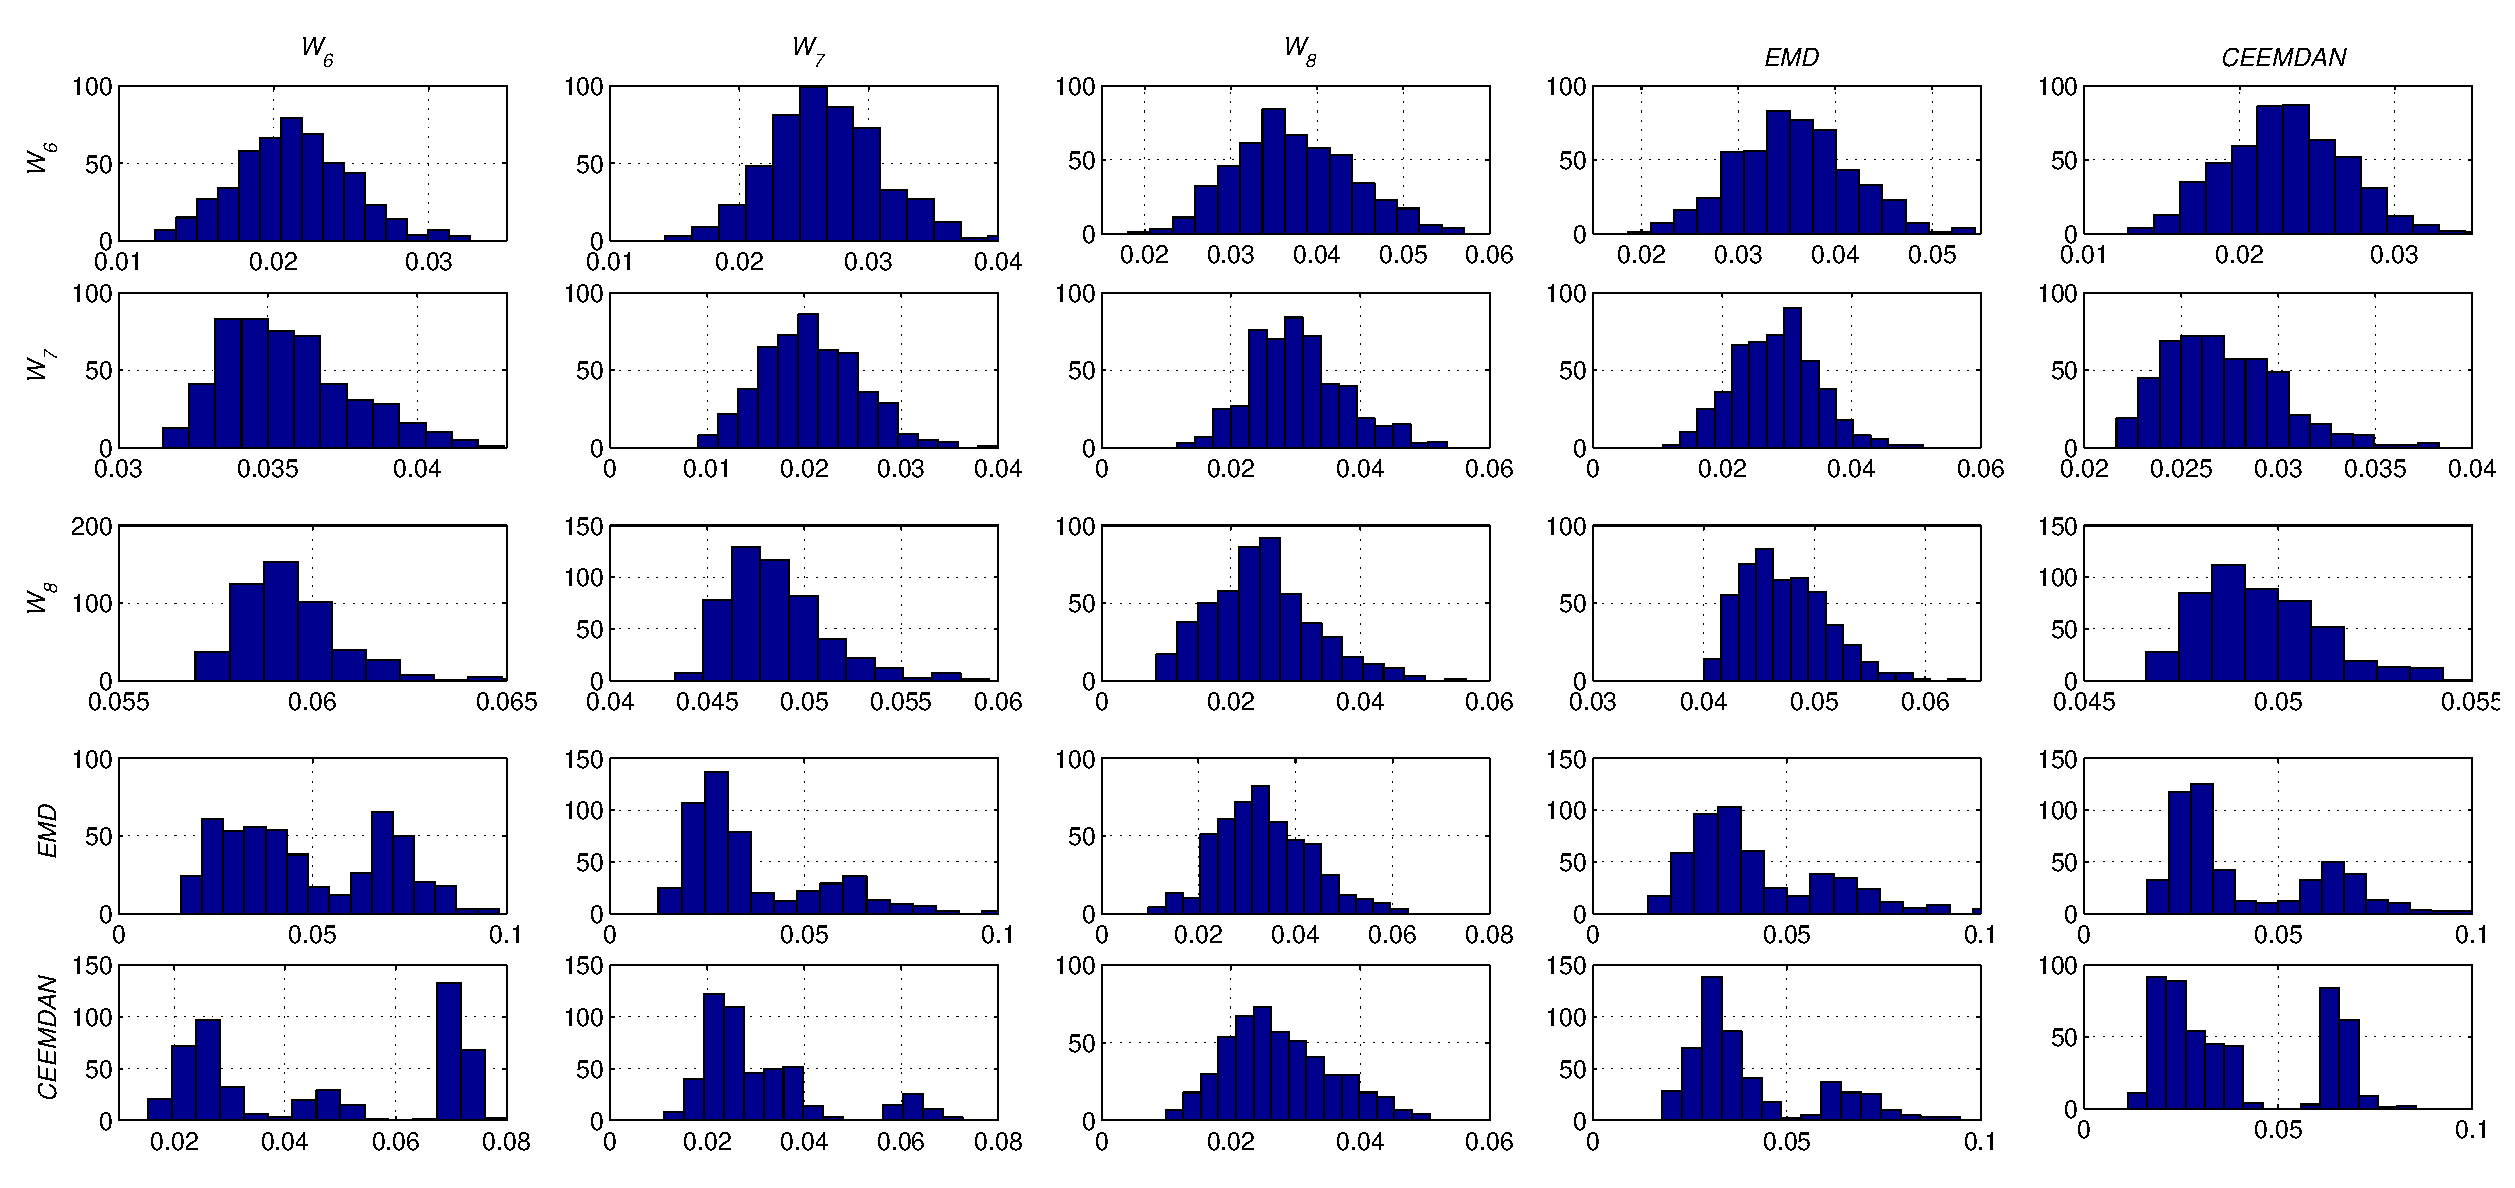
\includegraphics[width=1.0\textwidth,keepaspectratio]{Figure}
\caption{Название рисунка.}
\label{fig:}
\end{figure*}


% \appendix
% \section{Название приложения}
\label{sec:Appendix_}

Здесь размещается содержимое приложений к работе. В общем случае их может быть более одного.

\end{document}
